\begin{figure}[t]
	\centering
	\begin{subfigure}{0.31\textwidth}
		\centering
		\includegraphics[width=\textwidth]{figures/K2-posterior-W.pdf}
		% \caption{K2 ($F$: 0.9404)}
		\caption{K2}
	\end{subfigure}
	\begin{subfigure}{0.31\textwidth}
		\centering
		\includegraphics[width=\textwidth]{figures/K6-posterior-W.pdf}
		% \caption{K6 ($F$: 0.8742)}
		\caption{K6}
	\end{subfigure}
	\begin{subfigure}{0.31\textwidth}
		\centering
		\includegraphics[width=\textwidth]{figures/K7-posterior-W.pdf}
		% \caption{K7 ($F$: 0.9359)}
		\caption{K7}
	\end{subfigure}
	\begin{subfigure}{0.31\textwidth}
		\centering
		\includegraphics[width=\textwidth]{figures/K8-posterior-W.pdf}
		% \caption{K8 ($F$: 0.8645)}
		\caption{K8}
	\end{subfigure}
	\begin{subfigure}{0.31\textwidth}
		\centering
		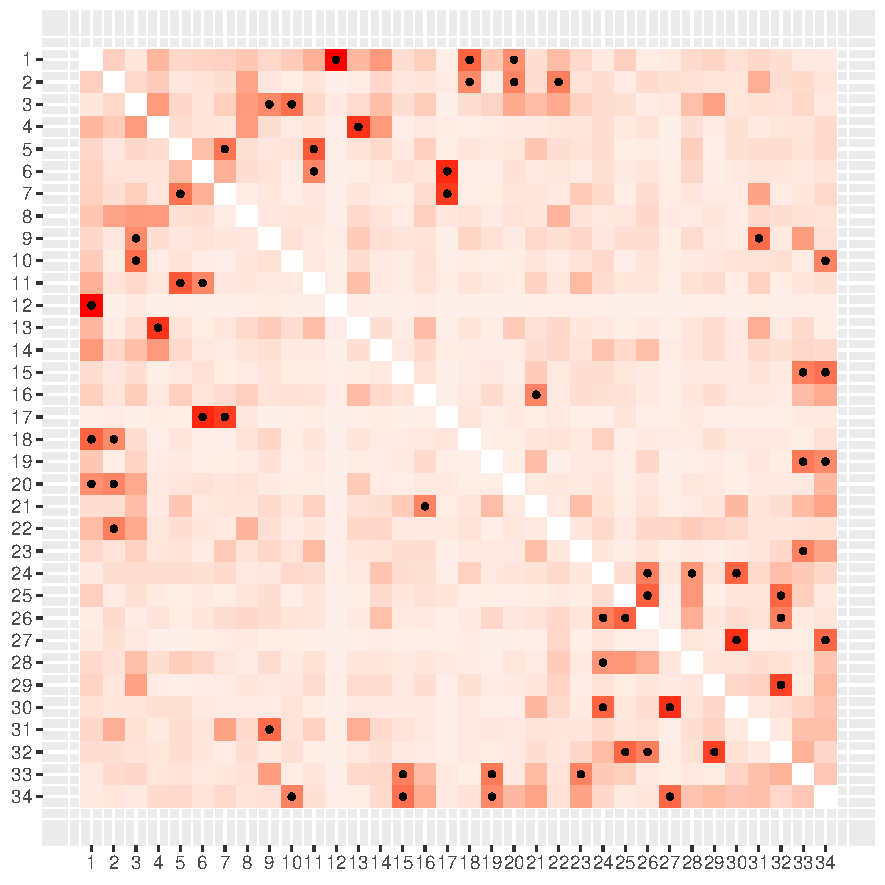
\includegraphics[width=\textwidth]{figures/K11-posterior-W.pdf}
		% \caption{K11 ($F$: 0.8366)}
		\caption{K11}
	\end{subfigure}
	\begin{subfigure}{0.31\textwidth}
		\centering
		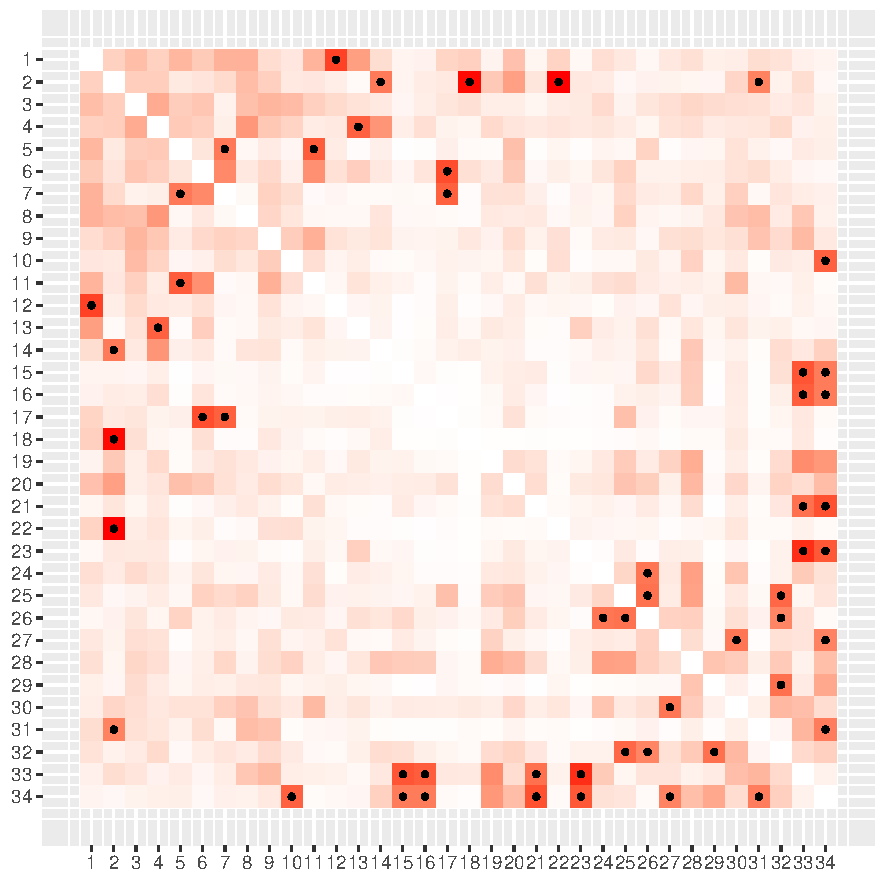
\includegraphics[width=\textwidth]{figures/K12-posterior-W.pdf}
		% \caption{K12 ($F$: 0.8497)}
		\caption{K12}
	\end{subfigure}
	\caption{Posterior Adjacency Matrices.}
	\label{fig:K-posterior-2}
\end{figure}
